\chapter{Векторна алгебра}

\section{Вектори на прямій, на площині, у просторі}

\begin{definition}
	\textbf{Вектор} --- це направлений відрізок прямої.
\end{definition}

Вектор повністю задається довжиною та напрямком. Також вектор можна
задати, вказавши його початок і кінець.

\noindent\parbox{1.3cm}{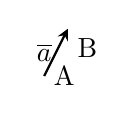
\begin{tikzpicture}[scale=0.3]  % vector image
	\draw[-stealth, thick] (1,0) -- (2,2);
	\draw (1,0) node[right]{A};
	\draw (2,2) node[below right]{B};
	\draw (1,1) node{$\overline{a}$};
\end{tikzpicture}}
\parbox{\textwidth - 1.4cm}{
	Вектори позначаються: $\overline{AB}, \overline{a}$, a їх довжини --- $|\overline{AB}|$, $|\overline{a}|$.
}

\begin{definition}
	Два \textbf{вектори рівні}, якщо їх довжини і напрямки співпадають.
\end{definition}

\noindent\parbox{2cm}{
	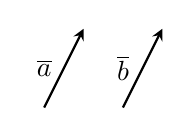
\begin{tikzpicture}[scale=0.5]
		\draw[-stealth, thick] (1,0) -- (2,2);
		\draw (1,1) node{$\overline{a}$};
		\draw[-stealth, thick] (3,0) -- (4,2);
		\draw (3,1) node{$\overline{b}$};
	\end{tikzpicture}
}
\parbox{\textwidth - 2.1cm}{
	$\overline{a} = \overline{b} \Leftrightarrow \overline{a} \upuparrows \overline{b}$
	(напрямки співпадають) та $|\overline{a}| = |\overline{b}|$ (довжини співпадають).
}

\begin{definition}
	\textbf{Колінеарні вектори} (паралельні вектори) $(\overline{a} \parallel \overline{b})$
	--- це вектори $\overline{a}$ і $\overline{b}$, які лежать на одній прямій або на паралельних прямих.
\end{definition}

Серед них будемо розрізняти вектори одного напрямку: $\overline{a} \upuparrows \overline{b}$, та протилежного напрямку: $\overline{a} \uparrow \downarrow \overline{b}$.

\begin{definition}
	\textbf{Нульовий вектор} (нуль - вектор) – це вектор нульової довжини, тобто вектор, кінець і початок якого співпадають, $|\overline{0}| = 0$. Буде зручно вважати нульовий вектор вектором довільного напрямку, тобто нульовий вектор є колінеарним будь-якому вектору.
\end{definition}

\begin{definition}
	Вектор $\overline{a}'$ --- \textbf{протилежний вектор} до вектора $\overline{a}$ , якщо $\overline{a}' \uparrow \downarrow \overline{a}$ і $|\overline{a}'| = |\overline{a}|$, тобто $\overline{a}' = -\overline{a}$.
\end{definition}

\begin{definition}
	Вектори $\overline{a}, \overline{b}, \overline{c}, ...$ --- це \textbf{компланарні вектори}, якщо вони лежать в одній площині або паралельні одній площині.
\end{definition}

\section{Лінійні операції над векторами}

\subsection*{Множення вектора на скаляр}

\begin{definition}
	\textbf{Добуток} вектора $\overline{a} \neq \overline{0}$  і числа $\alpha \in \mathbb{R}$, ($\alpha \overline{a}$) --- це вектор $\overline{b} = \alpha \overline{a}$, який задовольняє такі умови:
		\begin{enumerate}[label=\arabic*)]
			\item $\overline{b}$ колінеарний вектору $\overline{a}$
			\item $|\overline{b}| = |\alpha| |\overline{a}|$
			\item $\overline{b} \upuparrows \overline{a}$ --- однаково направлені, якщо $\alpha > 0$, і $\overline{b} \uparrow \downarrow \overline{a}$ – протилежно направлені, якщо $\alpha < 0$.
		\end{enumerate}
\end{definition}

\subsection*{Додавання векторів}

\begin{definition}
	\textbf{Сума векторів} $\overline{a}$ і $\overline{b}$, ($\overline{a} + \overline{b}$) --- це вектор, який з’єднує початок вектора $\overline{a}$ з кінцем вектора $\overline{b}$ за умови, що вектор $\overline{b}$ відкладено від кінця вектора $\overline{a}$.
\end{definition}

Цей спосіб додавання векторів --- це \textbf{правило трикутника}.

Два вектори можна додати і за іншим правилом, яке має назву --- \textbf{правило паралелограма}:
сумою двох векторів $\overline{a}$ і $\overline{b}$, відкладених від спільного початку, є
вектор, який збігається з діагоналлю паралелограма, побудованого на векторах $\overline{a}$
і $\overline{b}$ як на сторонах. Початки векторів $\overline{a}$, $\overline{b}$ та
$\overline{a} + \overline{b}$ співпадають.

\begin{center}
	\parbox{3cm}{
		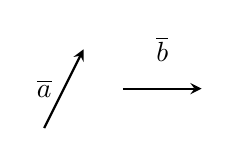
\begin{tikzpicture}[scale=0.5]  % vector a
			\draw[-stealth, thick] (0,1) -- (1,3);
			\draw (0,2) node{$\overline{a}$};
			\draw[-stealth, thick] (2,2) -- (4,2);
			\draw (3,3) node{$\overline{b}$};
		\end{tikzpicture}
	}
	\parbox{3cm}{
		\begin{tikzpicture}[scale=0.5]  %triangle rule
			\draw[-stealth, thick] (0,0) -- (1,2);
			\draw (0,1) node{$\overline{a}$};
			\draw[-stealth, thick] (1,2) -- (3,2);
			\draw (2,2.5) node{$\overline{b}$};
			\draw[-stealth, dashed, thick] (0,0) -- (3,2);
			\draw (2,0.5) node{$\overline{a} + \overline{b}$};
			\draw (1.5,-1) node{Правило};
			\draw (1.5,-2) node{трикутника};
		\end{tikzpicture}
	}
	\parbox{3cm}{			
		\begin{tikzpicture}[scale=0.5]  % paralelogram rule
			\draw[-stealth, thick] (0,0) -- (1,2);
			\draw (0,1) node{$\overline{a}$};
			\draw[-stealth, thick] (0,0) -- (2,0);
			\draw (1.5,0.5) node{$\overline{b}$};
			\draw[-stealth, thick] (0,0) -- (3,2);
			\draw (4,2) node{$\overline{a} + \overline{b}$};
			\draw[-stealth, dashed, thick] (1,2) -- (3,2);
			\draw[-stealth, dashed, thick] (2,0) -- (3,2);
			\draw (2,-1) node{Правило};
			\draw (2,-2) node{паралелограма};
		\end{tikzpicture}
	}
\end{center}

Використовуючи послідовно правило трикутника, можна побудувати суму скінченної
кількості довільних векторів. Якщо кінець останнього вектора співпадає з
початком першого, то сумою векторів є нульовий вектор: $\overline{0}$.

\begin{center}
	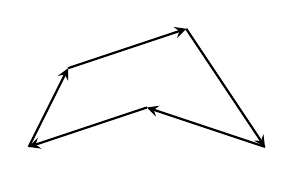
\begin{tikzpicture}[scale=0.5]  %triangle rule
		\draw[-stealth, thick] (0,0) -- (1,2);
		\draw[-stealth, thick] (1,2) -- (4,3);
		\draw[-stealth, thick] (4,3) -- (6,0);
		\draw[-stealth, thick] (6,0) -- (3,1);
		\draw[-stealth, thick] (3,1) -- (0,0);
	\end{tikzpicture}
\end{center}

\subsection*{Віднімання векторів}
 
\begin{definition}
	\textbf{Різниця векторів} $\overline{a}$ і $\overline{b}$, ($\overline{a} - \overline{b}$) --- це вектор $\overline{c}$, який в сумі з вектором $\overline{b}$ дає вектор $\overline{a}$ , тобто $\overline{b} + \overline{c} = \overline{a}$. 
\end{definition}

Очевидно, що $\overline{c} = \overline{a} + (-\overline{b})$.

\begin{center}
	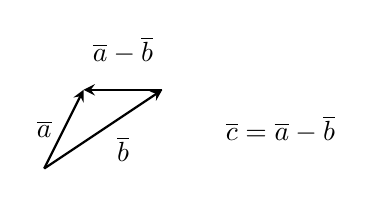
\begin{tikzpicture}[scale=0.5]  % paralelogram rule
		\draw[-stealth, thick] (0,0) -- (1,2);
		\draw (0,1) node{$\overline{a}$};
		\draw[-stealth, thick] (3,2) -- (1,2);
		\draw (2,3) node{$\overline{a} - \overline{b}$};
		\draw[-stealth, thick] (0,0) -- (3,2);
		\draw (2,0.5) node{$\overline{b}$};
		\draw (6,1) node{$\overline{c} = \overline{a} - \overline{b}$};
	\end{tikzpicture}
\end{center}

\parbox{\textwidth - 0.6cm}{\section{Властивості лінійних операцій, аксіоми векторної алгебри}}

\begin{enumerate}
	\item $(\alpha \beta) \overline{a} = \alpha (\beta \overline{a})$ --- асоціативність відносно множення на скаляр.

 	\item $\overline{a} + \overline{b} = \overline{b} + \overline{a}$ --- комутативність додавання.

 	\item $(\overline{a} + \overline{b}) + \overline{c} = \overline{a} + (\overline{b} + \overline{c})$ --- асоціативність додавання.
	
	\item \parbox[t]{8cm}{
		$\left.\begin{array}{l}
			(\alpha + \beta)\overline{a} = \alpha\overline{a} + \beta\overline{a}  \\
			\overline{a}(\alpha + \beta) = \overline{a}\alpha + \overline{a}\beta
		\end{array} \right\}$ --- дистрибутивність.
	}
	
	\item $\exists! \overline{0}: \forall\overline{a}: \overline{a} + \overline{0} = \overline{a}$ --- існування єдиного нуля.
    
    \item $\forall\overline{a} \exists!\overline{a}': \overline{a}' + \overline{a} = \overline{0}$ --- існування протилежного вектора.
    
    \item $1\cdot\overline{a} = \overline{a}$    
\end{enumerate}

\section{Базис на прямій, на площині, у просторі}

Розглянемо множину векторів, колінеарних вектору $\overline{a} \neq \overline{0}$. Позначимо її $E^1$.

Нехай $\overline{a}, \overline{b}, \overline{c} \in E^1$.

\begin{center}
	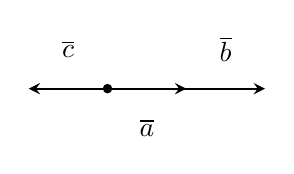
\begin{tikzpicture}[scale=0.5]
		\draw[-stealth, thick] (2,0) -- (0,0);
		\draw (1,1) node{$\overline{c}$};
		\filldraw[black] (2,0) circle (3pt);
		\draw[-stealth, thick] (2,0) -- (4,0);
		\draw (3,-1) node{$\overline{a}$};
		\draw[-stealth, thick] (2,0) -- (6,0);
		\draw (5,1) node{$\overline{b}$};
	\end{tikzpicture}
\end{center}

\begin{theorem} \label{vectorSingleRepresentation}
	$\forall \overline{b} \in E^1 \exists$ дійсне число $\alpha$ таке, що $\overline{b} = \alpha\overline{a}$, причому це представлення єдине. 
\end{theorem}
\begin{proof}
	Доведемо єдиність даного представлення методом від супротивного.
	
	Нехай $\overline{b} = \tilde{\alpha}\overline{a}$
	
	Тоді $\overline{0} = \overline{b} - \overline{b} = \tilde{\alpha}\overline{a} - \alpha\overline{a} = (\tilde{\alpha} - \alpha)\overline{a} \Rightarrow \tilde{\alpha} - \alpha = 0 \Rightarrow \tilde{\alpha} = \alpha$ 

	Вкажемо значення коефіцієнта $\alpha$.
	
	Якщо $\overline{a} \upuparrows \overline{b}$, то $\alpha = \dfrac{|\overline{b}|}{|\overline{a}|}$.
	
	Дійсно: $|\alpha\overline{a}| = \left|\dfrac{|\overline{b}|}{|\overline{a}|}\right||\overline{a}| = \dfrac{|\overline{b}|}{|\overline{a}|}|\overline{a}| = |\overline{b}|$, $\alpha\overline{a} \upuparrows \overline{b}$.

	Якщо ж $\overline{a} \uparrow \downarrow \overline{b}$, то $\alpha = -\dfrac{|\overline{b}|}{|\overline{a}|}$ (доведення аналогічне).
\end{proof}

Нехай $\overline{a} \nparallel \overline{b}$ ( тому $\overline{a} \neq \overline{0}$, $\overline{b} \neq \overline{0}$). Розглянемо множину векторів, компланарних векторам $\overline{a}$ та $\overline{b}$, позначимо її $E^2$.
Нехай $\overline{a}, \overline{b}, \overline{c} \in E^2$.

\begin{theorem}
	$\forall \overline{c} \in E^2 ~ \exists!$  дійсні $\alpha, \beta$, такі, що $\overline{c} = \alpha\overline{a} + \beta\overline{b}$.
\end{theorem} 

\begin{proof}
	Проведемо доведення графічно. 

	\begin{wrapfigure}{r}{4cm}
		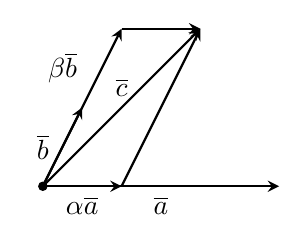
\begin{tikzpicture}[scale=0.5]
			\draw[-stealth, thick] (0,0) -- (1,2);
			\draw[-stealth, thick] (0,0) -- (2,4);
			\draw[-stealth, thick] (0,0) -- (2,0);
			\draw[-stealth, thick] (2,4) -- (4,4);
			\draw[-stealth, thick] (0,0) -- (4,4);
			\draw[-stealth, thick] (2,0) -- (4,4);
			\draw[-stealth, thick] (0,0) -- (6,0);
			\draw (0,1) node{$\overline{b}$};
			\draw (0.5,3) node{$\beta\overline{b}$};
			\draw (1,-0.5) node{$\alpha\overline{a}$};
			\draw (3,-0.5) node{$\overline{a}$};
			\draw (2,2.5) node{$\overline{c}$};
			\filldraw[black] (0,0) circle (3pt);
		\end{tikzpicture}
	\end{wrapfigure}
	
	З кінця вектору $\overline{c}$ проведемо дві прямі паралельно векторам $\overline{a}$ і $\overline{b}$ відповідно до перетину з цими векторами чи прямими, на яких вони лежать. 
	Отримали паралелограм, дві сторони якого дорівнюють відповідно $\alpha\overline{a}$ і $\beta\overline{b}$ (за теоремою~\ref{vectorSingleRepresentation}).
	Діагоналлю цього паралелограма є вектор $\overline{c}$, тобто $\overline{c} = \alpha\overline{a} + \beta\overline{b}$.
	Єдиність коефіцієнтів $\alpha$ та $\beta$ випливає з двох умов: 
	
	1) існує лише одна точка перетину непаралельних прямих, 
	
	2) за теоремою~\ref{vectorSingleRepresentation} константи $\alpha$ і $\beta$ визначаються однозначно.

\end{proof}

Нехай $E^3$ --- множина всіх векторів у просторі, причому $\overline{a}, \overline{b}, \overline{c}$ --- некомпланарні $(\overline{a} \neq \overline{0}, \overline{b} \neq \overline{0}, \overline{c} \neq \overline{0})$.

\begin{theorem}
	$\forall\overline{d}\in E^3, \exists! ~ \alpha, \beta, \gamma : \overline{d} = \alpha\overline{a} + \beta\overline{b} + \gamma\overline{c}$.
\end{theorem}

\newpage

\begin{proof}

	\begin{wrapfigure}{l}{4.2cm}
		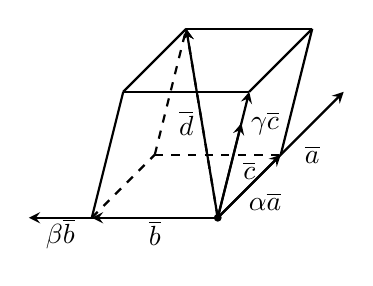
\begin{tikzpicture}[scale=0.4]
			\draw[-stealth, thick] (6,1) -- (2,1);
			\draw[-stealth, thick] (6,1) -- (0,1);
			\draw[-stealth, thick] (6,1) -- (5,7);
			\draw[-stealth, thick] (6,1) -- (6.75,4);
			\draw[-stealth, thick] (6,1) -- (7,5);
			\draw[-stealth, thick] (6,1) -- (8,3);
			\draw[-stealth, thick] (6,1) -- (10,5);
					
			\draw[thick] (2,1) -- (3,5);
			\draw[thick] (3,5) -- (5,7);
			\draw[thick] (3,5) -- (7,5);
			\draw[thick] (5,7) -- (9,7);
			\draw[thick] (7,5) -- (9,7);
			\draw[thick] (8,3) -- (9,7);
		
			\draw[thick, dashed] (2,1) -- (4,3);
			\draw[thick, dashed] (4,3) -- (5,7);
			\draw[thick, dashed] (4,3) -- (8,3);
			\draw[-stealth, dashed, thick] (6,1) -- (5,7);
			
			\draw (1,0.5) node{$\beta\overline{b}$};
			\draw (4,0.5) node{$\overline{b}$};
			\draw (5,4) node{$\overline{d}$};
			\draw (7,2.5) node{$\overline{c}$};
			\draw (7.5,4) node{$\gamma\overline{c}$};
			\draw (7.5,1.5) node{$\alpha\overline{a}$};
			\draw (9,3) node{$\overline{a}$};
			\filldraw[black] (6,1) circle (3pt);
		\end{tikzpicture}
	\end{wrapfigure}
		
	Із кінця вектора $\overline{d}$ проведемо три площини, паралельні парам
	векторів $(\overline{b}, \overline{c})$, $(\overline{a}, \overline{c})$, $(\overline{a}, \overline{b})$. Ці площини перетнуть прямі, на яких лежать $\overline{a}, \overline{b}, \overline{c}$ в
	єдиних точках.
	За теоремою~\ref{vectorSingleRepresentation} отримаємо нові вектори
	$\alpha\overline{a}, \beta\overline{b}, \gamma\overline{c}$, а вектор $\overline{d}$ – це діагональ
	паралелепіпеда, на них побудованого,
	тобто $\overline{d} = \alpha\overline{a} + \beta\overline{b} + \gamma\overline{c}$, що і треба було
	довести.

\end{proof}

\begin{remark}
	Базисом у множині $E^1$ може слугувати довільний ненульовий
	вектор, базисом у $E^2$ – впорядкована пара неколінеарних векторів, а в $E^3$ ---
	впорядкована трійка некомпланарних векторів. Вектору $\overline{b}$ було поставлено у
	відповідність число $\alpha$; вектору $\overline{c}$ – числа $\alpha$ і $\beta$; вектору 
	$\overline{d}$ – числа $\alpha, \beta, \gamma$. 
	Ці числа називаються --- коефіцієнти розкладу векторів $\overline{b}, \overline{c}, \overline{d}$ за базисами
	$\overline{a}$; $\overline{a}, \overline{b}$; $\overline{a}, \overline{b}, \overline{c}$ просторів $E^1, E^2$ і $E^3$ відповідно.
\end{remark}

\begin{definition}	
	\textbf{Коефіцієнти розкладу вектора $\overline{a}$ за базисом $\overline{a}_1, \overline{a}_2, ...$} --- це числа $\alpha_1, \alpha_2, ... \in \mathbb{R}$, такі, що $\overline{a} = \alpha_1\overline{a}_1 + \alpha_2\overline{a}_2 + ...$.
\end{definition}

\section{Декартів прямокутний базис}

\begin{definition}
	Впорядкована трійка некомпланарних векторів $(\overline{a}, \overline{b}, \overline{c})$ називається правою (\textbf{права трійка векторів}),
	якщо з кінця вектора $\overline{c}$ поворот від $\overline{a}$ до $\overline{b}$, менший за $180^{\circ}$, тобто відбувається проти
	годинникової стрілки.
\end{definition}

\begin{definition}
	Трійка векторів $\overline{i}, \overline{j}, \overline{k}$ утворює \textbf{декартів правий прямокутний базис}, якщо: 
	\begin{enumerate}
		\item $\overline{i} \perp \overline{j}, \overline{j} \perp \overline{k}, \overline{k} \perp \overline{i}$
		\item $|\overline{i}| = |\overline{j}| = |\overline{k}| = 1$
		\item $\overline{i}, \overline{j}, \overline{k}$ --- права трійка
	\end{enumerate}
\end{definition}

\section{Проекція вектора на вектор (або на вісь)}

Нехай задано $\overline{a} \neq \overline{0}$.

\begin{definition}
	\textbf{Проекція вектора $\overline{AB}$ на вектор $\overline{a}$} називається довжина відрізка $A'B'$ між основами перпендикулярів, опущених з точок A та B на вектор $\overline{a}$ (або напряму, на якій він лежить): 
\end{definition}

\begin{center}
	\parbox{4cm}{
		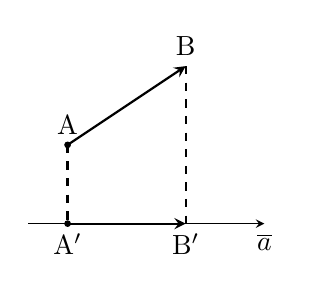
\begin{tikzpicture}[scale=0.5]
			\draw[-stealth] (0,0) -- (6,0)node[below]{$\overline{a}$};
			\draw[-stealth, thick] (1,2)node[above]{A} -- (4,4)node[above]{B};
			\filldraw[black] (1,2) circle (2pt);
			\draw[-stealth, thick] (1,0)node[below]{A$'$} -- (4,0)node[below]{B$'$};
			\filldraw[black] (1,0) circle (2pt);	
			\draw[dashed, thick] (1,2) -- (1,0);
			\draw[dashed, thick] (4,4) -- (4,0);
		\end{tikzpicture}
	}
	\parbox{6.2cm}{
		$\text{пр}_{\overline{a}}\overline{AB} = \left\{ \begin{array}{l}
			|\overline{A'B'}| \text{, якщо } \overline{A'B'}\uparrow\uparrow \overline{a}  \\
			-|\overline{A'B'}|\text{, якщо } \overline{A'B'}\uparrow\downarrow\overline{a}  \\
		\end{array}\right.$
	}
\end{center}

\subsection*{Властивості проекції:}
\begin{enumerate}
	\item $\text{пр}_{\overline{a}}\alpha\overline{b} = \alpha\text{пр}_{\overline{a}}\overline{b}$
	\item $\text{пр}_{\overline{a}}(\overline{a} + \overline{b}) = \text{пр}_{\overline{a}}\overline{a} + \text{пр}_{\overline{a}}\overline{b}$
\end{enumerate}

\section{Множення векторів. Скалярний добуток двох векторів}

\begin{definition}
	\textbf{Скалярний добуток} векторів $\overline{a}$ і $\overline{b}$ (позначається
	$\overline{a}\cdot\overline{b}$, $\overline{a}\overline{b}$ чи $(\overline{a}, \overline{b})$)
	--- це число, яке дорівнює добутку довжин цих векторів на косинус кута між ними: 
	$(\overline{a}, \overline{b}) = |\overline{a}||\overline{b}|\cos\varphi$, де
	$\varphi = \widehat{(\overline{a}, \overline{b})}$.
\end{definition}

\subsection*{Алгебраїчні властивості скалярного добутку:}
\begin{enumerate}
	\item $(\overline{a}, \overline{b}) = (\overline{b}, \overline{a})$ --- комутативність.
	\item $\left.\begin{array}{l}
				(\alpha\overline{a}, \overline{b}) = \alpha(\overline{a}, \overline{b}) = (\overline{a}, \alpha\overline{b})  \\
				(\overline{a} + \overline{a}', \overline{b}) = (\overline{a}, \overline{b}) + (\overline{a}', \overline{b})  \\
				(\overline{a}, \overline{b} + \overline{b}') = (\overline{a}, \overline{b}) + (\overline{a}, \overline{b}')  \\
		  \end{array}\right\}$ --- лінійність.
\end{enumerate}

\subsection*{Геометричні властивості скалярного добутку:}
\begin{enumerate}
	\item $(\overline{a}, \overline{b}) = 0 \Leftrightarrow \overline{a} \perp \overline{b}$.
	\item $(\overline{a}, \overline{a}) = |\overline{a}|^2 \Rightarrow |\overline{a}| = \sqrt{(\overline{a}, \overline{a})}$.
\end{enumerate}

\section{Скалярний добуток в координатах}

Нехай $\{\overline{e}_1, \overline{e}_2, \overline{e}_3\}$ – це фіксований базис в просторі $E^3$,
$\overline{x}, \overline{y} \in E^3$. Тоді:
\begin{center}
	$\overline{x} = x_1\overline{e}_1 + x_2\overline{e}_2 + x_3\overline{e}_3$  \\
	$\overline{y} = y_1\overline{e}_1 + y_2\overline{e}_2 + y_3\overline{e}_3$  \\
\end{center}

Обчислимо скалярний добуток цих векторів: 

\noindent\parbox{\textwidth}{\raggedright$(\overline{x}, \overline{y})
= (x_1\overline{e}_1 + x_2\overline{e}_2 + x_3\overline{e}_3, \overline{y})
= (x_1 \overline{e}_1, \overline{y}) + (x_2 \overline{e}_2, \overline{y})
+ (x_3 \overline{e}_3, \overline{y})
= x_1(\overline{e}_1, y_1\overline{e}_1 + y_2\overline{e}_2 + y_3\overline{e}_3)
+ x_2(\overline{e}_2, y_1\overline{e}_1 + y_2\overline{e}_2 + y_3\overline{e}_3)
+ x_3(\overline{e}_3, y_1\overline{e}_1 + y_2\overline{e}_2 + y_3\overline{e}_3)
= x_1 y_1(\overline{e}_1, \overline{e}_1)
+ x_1 y_2(\overline{e}_1, \overline{e}_2)
+ x_1 y_3(\overline{e}_1, \overline{e}_3)
+ x_2 y_1(\overline{e}_2, \overline{e}_1)
+ x_2 y_2(\overline{e}_2, \overline{e}_2)
+ x_2 y_3(\overline{e}_2, \overline{e}_3)
+ x_3 y_1(\overline{e}_3, \overline{e}_1)
+ x_3 y_2(\overline{e}_3, \overline{e}_2)
+ x_3 y_3(\overline{e}_3, \overline{e}_3)
= x_1 y_1(\overline{e}_1, \overline{e}_1)
+ (x_1 y_2 + x_2 y_1)(\overline{e}_1, \overline{e}_2)
+ (x_1 y_3 + x_3 y_1)(\overline{e}_1, \overline{e}_3)
+ x_2 y_2(\overline{e}_2, \overline{e}_2)
+ (x_2 y_3 + x_3 y_2)(\overline{e}_2, \overline{e}_3)
+ x_3 y_3(\overline{e}_3, \overline{e}_3).$}

У частковому випадку, коли $\overline{e}_1 = \overline{i}, \overline{e}_2 = \overline{j}, \overline{e}_3 = \overline{k}$, маємо: 
$(\overline{e}_1, \overline{e}_2) = (\overline{e}_2, \overline{e}_3) = (\overline{e}_3, \overline{e}_1), (\overline{e}_i, \overline{e}_j) = 1$, де $i = 1, 2, 3$.

$$(\overline{x}, \overline{y}) = x_1 y_1 + x_2 y_2 + x_3 y_3$$

Якщо $\overline{a} = (x, y, z)$, то $|\overline{a}| = \sqrt{(\overline{a}, \overline{a})} = \sqrt{x^2 + y^2 + z^2}$.

\section{Нормування вектора}

\begin{definition}
	Нехай $\overline{a} \neq \overline{0}$. \textbf{Орт-вектор} вектора $\overline{a}$ --- це вектор $\overline{a}_o$, такий, що $\overline{a}_o \uparrow\uparrow \overline{a}$ і $|\overline{a}_o| = 1$. 
\end{definition}

\begin{definition}
	 \textbf{Нормування вектора} $\overline{a}$ --- це процес отримання орт-вектора $\overline{a}_o$, $\overline{a}_o = \dfrac{1}{|\overline{a}|}\overline{a}$
\end{definition}

Якщо $\overline{a} = (x, y, z)$, то
$$\overline{a}_o = \left(\dfrac{x}{\sqrt{x^2+y^2+z^2}}, \dfrac{y}{\sqrt{x^2+y^2+z^2}}, \dfrac{z}{\sqrt{x^2+y^2+z^2}} \right).$$

Геометричний сенс координат орт-вектора $\overline{a}_o$ у декартовій системі координат:
$\overline{a}_o = (\cos\alpha, \cos\beta, \cos\gamma)$ де, $\alpha = \widehat{(\overline{a}, OX)} = \widehat{(\overline{a}_o, OX)}$, $\beta = \widehat{(\overline{a}, OY)} = \widehat{(\overline{a}_o, OY)}$, $\gamma = \widehat{(\overline{a}, OZ)} = \widehat{(\overline{a}_o, OZ)}$.

\begin{definition}
	Косинуси кутів, які утворює вектор (або його орт) з осями координат --- це \textbf{напрямні косинуси}.
\end{definition}

Знайдемо косинус кута $\alpha$: 
$$\cos\alpha = \dfrac{(\overline{a}, \overline{i})}{|\overline{a}||\overline{i}|} = \dfrac{x}{\sqrt{x^2+y^2+z^2}}$$

\begin{claim}
	$\cos^2\alpha + \cos^2\beta + \cos^2\gamma = 1$.
\end{claim}

Формула для довжини проекції вектора:
$$x = |\overline{a}|\cos\alpha = \text{пр}_{\overline{i}}\overline{a}$$

\section{Векторний добуток двох векторів}

\begin{definition}
	\textbf{Векторний добуток} векторів $\overline{a}$ і $\overline{b}$ $[\overline{a}, \overline{b}]$
	--- це вектор $\overline{c}$, що задовольняє умови:
	\begin{enumerate}
		\item $\overline{c}\perp\overline{a}$, $\overline{c}\perp\overline{b}$
		\item $|\overline{a}| = |\overline{a}||\overline{b}|\sin\varphi$, $\varphi = (\widehat{\overline{a},
			\overline{b}})$
		\item $\overline{a}$, $\overline{b}$, $\overline{c}$ --- права трійка
	\end{enumerate}
\end{definition}

\begin{remark}
	Оскільки $\overline{c}\perp\overline{a}$, $\overline{c}\perp\overline{b}$, то $\overline{c}$
	перпендикулярний площині векторів $\overline{a}$ і $\overline{b}$. 
\end{remark}

\subsection*{Алгебраїчні властивості векторного добутку:}

1) $[\overline{a}, \overline{b}] = - [\overline{b}, \overline{a}]$
	
2) $[\alpha\overline{a}, \overline{b}] = \alpha[\overline{a}, \overline{b}] = [\overline{a}, \alpha\overline{b}]$

3) $[\overline{a} + \overline{b}, \overline{c}] = [\overline{a}, \overline{c}] + [\overline{b}, \overline{c}]$
	
4) $[\overline{a}, \overline{b} + \overline{c}] = [\overline{a}, \overline{b}] + [\overline{a}, \overline{c}]$

\textit{Доведення:}

\begin{proof}
	1) Нехай $[\overline{a}, \overline{b}] = \overline{c}$, $[\overline{b}, \overline{a}] = \overline{d}$.
	Тоді: $\overline{c} \perp \overline{a}$ і $\overline{c} \perp \overline{b}$,
	$\overline{d} \perp \overline{b}$ і $\overline{d} \perp \overline{a}$, тобто вектори $\overline{c}$
	і $\overline{d}$ перпендикулярні до площини, в якій лежать вектори $\overline{a}$ і $\overline{b}$,
	отже, $\overline{c} \parallel \overline{d}$.
	
	$|\overline{c}| = |\overline{a}||\overline{b}|\sin\varphi = |\overline{d}|$, де
	$\varphi = (\widehat{\overline{a},\overline{b}})$.
	
	$\overline{a}$, $\overline{b}$, $\overline{c}$ --- права трійка; $\overline{b}$, $\overline{a}$,
	$\overline{d}$ --- також права трійка $\Rightarrow$ $\overline{a}$, $\overline{b}$, $\overline{d}$
	--- ліва трійка, тому вектори $\overline{c}$ та $\overline{d}$ протилежно направлені.
	
	Отже, вектори $\overline{c}$ та $\overline{d}$ колінеарні, мають однакову довжину та протилежно
	направлені. Тому $\overline{c} = -\overline{d}$.

	~	
	
	2) Якщо $\alpha = 0$ або $\overline{a} \parallel \overline{b}$, то рівності очевидні: 
	$[\alpha \overline{a}, \overline{b}] = \alpha [\overline{a}, \overline{b}] = \overline{0}$.
	Нехай $\alpha < 0$, $[\overline{a}, \overline{b}] = \overline{c}$,
	$\varphi = (\widehat{\overline{a}, \overline{b}})$, $[\alpha \overline{a}, \overline{b}] = \overline{d}$.
	Тоді:
	
	$|\alpha \overline{c}| = |\alpha [\overline{a}, \overline{b}]| = |\alpha| |[\overline{a}, \overline{b}]|
	= -\alpha |\overline{a}| |\overline{b}| \sin\varphi$.
	
	$|[\alpha \overline{a}, \overline{b}]|
	= |\alpha \overline{a}| |\overline{b}]|\sin(\widehat{\alpha \overline{a},\overline{b}})
	= |\alpha| |\overline{a}| |\overline{b}]|\sin(\pi - \varphi)
	= -\alpha |\overline{a}| |\overline{b}]| \sin\varphi$.
	
	$\overline{c}\perp$ площині, в якій лежать $\overline{a}$ і $\overline{b}$
	$\Rightarrow \overline{c} \perp$ площині, в якій лежать $\alpha \overline{a}$ і $\overline{b}$.
	
	$\overline{d}\perp$ площині, в якій лежать $\alpha \overline{a}$ і $\overline{b}$, отже,
	$\overline{c} \parallel \overline{d}$.
	
	$\overline{a}$, $\overline{b}$, $\overline{c}$ --- права трійка $\alpha \overline{a}$,
	$\overline{b}$, $\overline{c}$ --- ліва трійка, $\overline{a}$, $\overline{b}$,
	$\alpha \overline{c}$ --- ліва трійка.
	
	$\alpha \overline{a}$, $\overline{b}$, $\overline{d}$ --- права трійка $\overline{a}$,
	$\overline{b}$, $\overline{d}$ --- ліва трійка; отже, вектори $\alpha \overline{c}$ та $\overline{d}$.
	однаково направлені.
	
	Враховуючи однакову довжину векторів $\alpha \overline{c}$ та $\overline{d}$, маємо
	$\alpha \overline{c} = \overline{d}$ або $[\alpha \overline{a}, \overline{b}]
	= \alpha [\overline{a}, \overline{b}]$.

	~

	3), 4) --- очевидно.
\end{proof}

\subsection*{Геометричні властивості векторного добутку:}

1) $[\overline{a}, \overline{b}] = \overline{0} \Leftrightarrow \overline{a} \parallel \overline{b}$

2) $|[\overline{a}, \overline{b}]| = S_{\Diamond \overline{a}\overline{b}}$, де
$S_{\Diamond \overline{a}\overline{b}}$ --- площа паралелограма, побудованого на векторах
$\overline{a}$ та $\overline{b}$ , як на сторонах

\textit{Доведення:}

\begin{proof}
	1) $|[\overline{a},\overline{b}]| = |\overline{a}| |\overline{b}| \sin\varphi = 0
	\Rightarrow \overline{a} = \overline{0}$ або $\overline{b} = \overline{0}$, або $\sin \varphi = 0
	\Rightarrow \overline{a} \parallel \overline{b}$.
	
	Якщо $\overline{a} \parallel \overline{b}$, то $\sin \varphi = 0$, і $|[\overline{a}, \overline{b}]| = 0
	\Rightarrow [\overline{a}, \overline{b}] = \overline{0}$.
	
	~	
	
	2) $|[\overline{a},\overline{b}]| = |\overline{a}| |\overline{b}| \sin \varphi = |\overline{a}| h
	= S_{\Diamond \overline{a}\overline{b}}$.
\end{proof}

\begin{claim}
	$[\overline{a}, \overline{a}] = 0$.
\end{claim}

\section{Векторний добуток в координатах}

Нехай в просторі $E^3$ зафіксовано базис $\{\overline{i}, \overline{j}, \overline{k}\}$, $\overline{x}, \overline{y} \in E^3$, тоді 

$$\overline{x} = x_1\overline{i} + y_1\overline{j} + z_1\overline{k}$$

$$\overline{y} = x_2\overline{i} + y_2\overline{j} + z_2\overline{k}$$

Знайдемо координати вектору $[\overline{x}, \overline{y}]$.

Зауважимо, що $[\overline{i}, \overline{j}] = \overline{k}$, $[\overline{j}, \overline{k}] = \overline{i}$,
$[\overline{k}, \overline{i}] = \overline{j}$. Тоді:

\noindent$[\overline{i}, \overline{j}]
= [x_1\overline{i} + y_1\overline{j} + z_1\overline{k}
	, x_2\overline{i} + y_2\overline{j} + z_2\overline{k}]
= x_1 x_2[\overline{i},\overline{i}]
	+ x_1 y_2[\overline{i},\overline{j}]
	+ x_1 z_2[\overline{i},\overline{k}]
	+ y_1 x_2[\overline{j},\overline{i}]
	+ y_1 y_2[\overline{j},\overline{j}]
	+ y_1 z_2[\overline{j},\overline{k}]
	+ z_1 x_2[\overline{k},\overline{i}]
	+ z_1 y_2[\overline{k},\overline{j}]
	+ z_1 z_2[\overline{k},\overline{k}]
= (x_1 y_2 - x_2 y_1)[\overline{i},\overline{j}]
	+ (x_1 z_2 - x_2 z_1)[\overline{i},\overline{k}]
	+ (y_1 z_2 - y_2 z_1)[\overline{j},\overline{k}]
= (x_1 y_2 - x_2 y_1)\overline{k}
	+ (x_1 z_2 - x_2 z_1)\overline{j}
	+ (y_1 z_2 - y_2 z_1)\overline{i}
= (y_1 z_2 - y_2 z_1)\overline{i}
	+ (x_1 z_2 - x_2 z_1)\overline{j}
	+ (x_1 y_2 - x_2 y_1)\overline{k}.$

\begin{problem}
	Знайти площу трикутника з вершинами $A(3, 0, -1)$, $B(-2, 4, 1)$, $C(2, 1, -3)$. 
\end{problem}
\begin{solution}
	$S = \dfrac{1}{2}|[\overline{AB},\overline{AC}]|$. Оскільки
	$\overline{AB} = (-5, 4, 2), \overline{AC} = (-1, 1, -2)$,
	то $[\overline{AB},\overline{AC}] = -10\overline{i} - 12\overline{j} - \overline{k}$.
	Тоді $|[\overline{AB},\overline{AC}]| = \sqrt{(-10)^2 + (-12)^2 + (-1)^2}
	= \sqrt{100 + 144 + 1} = \sqrt{245}$, і $S = \dfrac{1}{2}\sqrt{245}$
\end{solution}

\section{Мішаний добуток трьох векторів}

\begin{definition}
	\textbf{Мішаний добуток} векторів $\overline{a}, \overline{b}, \overline{c}$ --- це скалярний добуток $\overline{a}$
	з векторним добутком векторів $\overline{b}$ і $\overline{c}$, тобто $\overline{a}\overline{b}\overline{c} = (\overline{a}, [\overline{b}, \overline{c}])$. 
\end{definition}

\begin{theorem}
	Мішаний добуток векторів $\overline{a}, \overline{b}, \overline{c}$ дорівнює об’єму паралелепіпеда
	$V_{\text{пар}}$, побудованого на цих векторах, якщо вони складають праву трійку i дорівнює
	$-V_{\text{пар}}$, якщо $\overline{a}, \overline{b}, \overline{c}$ – ліва трійка:
	
	$$\overline{a}\overline{b}\overline{c} = \left\{\begin{array}{ll}
		V_{\text{пар}},		& \text{ якщо } \overline{a},\overline{b},\overline{c} \text{ --- права трійка}  \\
		-V_{\text{пар}},	& \text{ якщо } \overline{a},\overline{b},\overline{c} \text{ --- ліва трійка}  \\
	\end{array} \right.$$
\end{theorem}
\begin{proof}
	Розглянемо випадок, коли $\overline{a},\overline{b},\overline{c}$ --- права трійка.
	
	\begin{wrapfigure}{l}{4cm}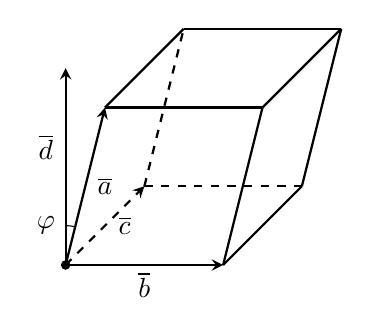
\begin{tikzpicture}[scale=0.5]
		\draw[-stealth, thick] (0,0) -- (0,5);
		\draw[-stealth, thick] (0,0) -- (1,4);
		\draw[-stealth, thick, dashed] (0,0) -- (2,2);
		\draw[-stealth, thick] (0,0) -- (4,0);
				
		\draw[thick] (1,4) -- (5,4);
		\draw[thick] (1,4) -- (3,6);
		\draw[thick] (5,4) -- (7,6);
		\draw[thick] (3,6) -- (7,6);
		\draw[thick] (4,0) -- (6,2);
		\draw[thick] (6,2) -- (7,6);
		\draw[thick] (4,0) -- (5,4);
			
		\draw[thick, dashed] (2,2) -- (3,6);
		\draw[thick, dashed] (2,2) -- (6,2);
				
		\filldraw[black] (0,0) circle (3pt);
				
		\draw (-0.5,3) node{$\overline{d}$};
		\draw (2,-0.5) node{$\overline{b}$};
		\draw (1.5,1) node{$\overline{c}$};
		\draw (1,2) node{$\overline{a}$};

		\draw[black] (0,1) arc (90:75.97:1);
		\draw (-0.5,1) node{$\varphi$};
	\end{tikzpicture}\end{wrapfigure}
	%\parbox[b]{8cm}{
		Нехай $[\overline{b}, \overline{c}] = \overline{d}$. Тоді $\overline{b}$, $\overline{c}$,
		$\overline{d}$ -- права трійка. Позначимо $\varphi = \widehat{(\overline{a}, \overline{d})}$.

		Тоді $\overline{a}\overline{b}\overline{c} = (\overline{a},[\overline{b},\overline{c}]) = (\overline{a},\overline{d}) = |\overline{a}||\overline{d}|\cos\varphi
		= S_{\Diamond \overline{c}\overline{b}}|\overline{a}|\cos\varphi = S_{\Diamond \overline{c}\overline{b}}h = V_{\text{пар}}$, оскільки висота
		паралелепіпеда $h = |\overline{a}|\sin\left(\dfrac{\pi}{2} - \varphi\right) = |\overline{a}|\cos\varphi$.
		У випадку, коли $\overline{a}, \overline{b}, \overline{c}$ --- ліва трійка, доведення
		аналогічне.%}

\end{proof}
%\vspace{20px}

\subsection*{Алгебраїчні властивості:}

\begin{enumerate}
	\item $\overline{a}\overline{b}\overline{c} = \overline{c}\overline{a}\overline{b} = \overline{b}\overline{c}\overline{a} = -\overline{b}\overline{a}\overline{c} = -\overline{c}\overline{b}\overline{a} = -\overline{a}\overline{c}\overline{b}$
	\item $(\alpha\overline{a})\overline{b}\overline{c} = \alpha\overline{a}\overline{b}\overline{c} = \overline{a}(\alpha\overline{b})\overline{c} = \overline{a}\overline{b}(\alpha\overline{c})$
	\item $\begin{array}{l}
			(\overline{a}+\overline{a}')\overline{b}\overline{c} = \overline{a}\overline{b}\overline{c} + \overline{a}'\overline{b}\overline{c}  \\
			\overline{a}(\overline{b}+\overline{b}')\overline{c} = \overline{a}\overline{b}\overline{c} + \overline{a}\overline{b}'\overline{c}  \\
			\overline{a}\overline{b}(\overline{c}+\overline{c}') = \overline{a}\overline{b}\overline{c} + \overline{a}\overline{b}\overline{c}'  \\
		\end{array}$	
\end{enumerate}

\textit{Доведення:}

\begin{proof}
	1) випливає з того факту, що при циклічній перестановці векторів їх
	орієнтація не змінюється. А якщо в трійці векторів деякі два з них поміняти
	місцями, то її орієнтація змінюється.

	~
	
	2) випливає з лінійності скалярного і векторного добутків відносно
	множення на скаляр.

	~

	3) $(\overline{a} + \overline{a}')\overline{b}\overline{c}
	= (\overline{a} + \overline{a}',[\overline{b},\overline{c}])
	= (\overline{a},[\overline{b},\overline{c}])
		+ (\overline{a}',[\overline{b},\overline{c}])
	= \overline{a}\overline{b}\overline{c} + \overline{a}'\overline{b}\overline{c}$

	$\overline{a}(\overline{b} + \overline{b}')\overline{c}
	= (\overline{b} + \overline{b}')\overline{c}\overline{a}
	= \overline{b}\overline{c}\overline{a} + \overline{b}'\overline{c}\overline{a}
	= \overline{a}\overline{b}\overline{c} + \overline{a}\overline{b}'\overline{c}.$
	
	Але $\overline{a}(\overline{b} + \overline{b}')\overline{a}
	= (\overline{a},[\overline{b} + \overline{b}',\overline{c}])
	= (\overline{a},[\overline{b}, \overline{c}] + [\overline{b}',\overline{c}]).$
	
	Ця рівність справедлива $\forall \overline{a}$. Тому $[\overline{b} + \overline{b}',\overline{c}]
	= [\overline{b},\overline{c}] + [\overline{b}',\overline{c}]$, що доводить
	властивість 3 векторного добутку.
\end{proof}

\begin{claim}
	$\overline{a} \overline{b} \overline{c}
	= (\overline{a},[\overline{b},\overline{c}])
	=([\overline{a},\overline{b}],\overline{c}).$
\end{claim}

\section{Мішаний добуток в координатах}

Нехай в просторі $E^3$ зафіксовано базис $\{\overline{i}, \overline{j}, \overline{k}\}$ і задано три вектори:

$\overline{a} = (a_1, a_2, a_3)$, $\overline{b} = (b_1, b_2, b_3)$, $\overline{c} = (c_1, c_2, c_3)$.

Тоді $[\overline{b}, \overline{c}]
= (b_2c_3-b_3c_2)\overline{i} - (b_1c_3-b_3c_1)\overline{j} + (b_1c_2-b_2c_1)\overline{k}$
та $\overline{a}\overline{b}\overline{c} = (\overline{a},[\overline{b},\overline{c}]) = a_1(b_2c_3-b_3c_2) - a_2(b_1c_3-b_3c_1) + a_3(b_1c_2-b_2c_1) = 
a_1b_2c_3 - a_1b_3c_2 - a_2b_1c_3 + a_2b_3c_1 + a_3b_1c_2 - a_3b_2c_1$.

\begin{problem}
	Чи можуть вектори $\overline{e}_1=(1,-1,0)$, $\overline{e}_2=(2,0,-2)$, $\overline{e}_3=(3,1,6)$ слугувати базисом в просторі $E^3$?
\end{problem}
\begin{solution}
	Якщо $\overline{e}_1, \overline{e}_2, \overline{e}_3$ --- базис, то вони некомпланарні і об’єм
	паралелепіпеда, на них побудованого, не дорівнює нулю. Тобто, $\overline{e}_1\overline{e}_2\overline{e}_3 \neq 0$.
	Знайдемо мішаний добуток $\overline{e}_1\overline{e}_2\overline{e}_3$:
	$\overline{e}_1\overline{e}_2\overline{e}_3 = 0 + 0 + 6 + 0 + 2 + 12 = 20 \neq 0$.
	Це означає, що дані вектори можуть слугувати базисом в $E^3$.
\end{solution}

